\documentclass[pdf]{article}
\usepackage{pgfplots} 
%\usepgfplotslibrary{external} 
%\tikzexternalize 
\usepgfplotslibrary{fillbetween}
\usepackage{tikz} 
\usepackage{amsmath} 
\usetikzlibrary{calc} 
\pgfplotsset{compat = newest, every axis plot post/.style={line join=round},every non boxed x axis/.append style={x axis line style=-}, every non boxed y axis/.append style={y axis line style=-}}
\begin{document} 
	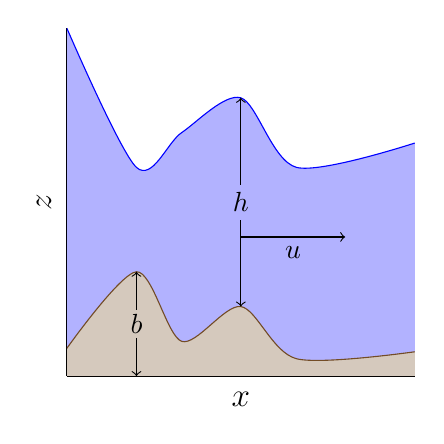
\begin{tikzpicture} 
	\begin{axis}[ 
	width = 0.7\textwidth,
	label style={font=\large},
	axis lines=left, xtick=\empty,
	ytick=\empty,
	clip mode=individual,
	xmin=0, 
	xmax=1, 
	width = 6cm,
	height = 6cm,
	ymin = 0, 
	ymax = 1,
	xlabel=$x$, 
	ylabel=$z$ ]
	%\addplot [blue] coordinates {(0,0.8)  (0.66,0.8)};
	\path[name path=axis] (axis cs:0,0) -- (axis cs:1,0);
	%\node[left] at (0,0.08) {$b$};
	\addplot [name path=b,brown!60!black, smooth] coordinates { (0,0.08) (0.2,0.3) (0.33,0.1) (0.5,0.2) (0.66,0.05) (1,0.07)};
	
	\addplot [
	thick,
	color=brown!60!black,
	fill=brown!60!black, 
	fill opacity=0.3
	] fill between[of=b and axis];
	
	
	%\node[left] at (0,0.9) {$h$};
	\addplot [name path=h,blue, smooth] coordinates { (0,1) (0.2,0.6) (0.33,0.7) (0.5,0.8) (0.66,0.6) (1,0.67)};
	
	\addplot [
	thick,
	color=blue,
	fill=blue, 
	fill opacity=0.3
	] fill between[of=h and b];
	
	
	\addplot [<-,black] coordinates {(0.5,0.2) (0.5,0.45)};
	\node[] at (0.5,0.5) {$h$};
	\addplot [->,black] coordinates {(0.5,0.55) (0.5,0.8)};
	
	\addplot [<-,black] coordinates {(0.2,0.3) (0.2,0.19)};
	\node[] at (0.2,0.15) {$b$};
	\addplot [->,black] coordinates {(0.2,0.11) (0.2,0)};
	
	
	\addplot [->,black] coordinates {(0.5,0.4) (0.8,0.4)};
	\node[below] at (0.65,0.4) {$u$};
	
	
	\end{axis} 
	\end{tikzpicture}  
\end{document}